\Exercise[number={10}]
Any binary classifier divides the \(x\) space into two regions,
\(\mathfrak{R}_1\) and \(\mathfrak{R}_2\). The probability of error is
defined by the sum of the propbability that the correct class is \(w_1\)
but \(x\) belongs to region \(\mathfrak{R}_2\) and the probability that
the correct class is \(w_2\) but \(x\) belongs to \(\mathfrak{R}_1\), i.e.
\(p(\text{error})=p(x\in\mathfrak{R}_2, w_1)+p(x\in\mathfrak{R}_1, w_2)\).
Suppose that \(x\) is defined in \(\mathbf{R}\) (scalar) and that both
\(p(x|w_i)\) have a Cauchy distribution:
\[
    p(x|w_i)=\frac{1}{\pi b}\frac{1}{1+\bigl(\frac{x-a_i}{b}\bigr)^2}
\]
with \(a_2>a_1\). Also assume that \(Pr(w_1)=Pr(w_2)=0.5\).\\
a. Define a Bayes classifier, and determine the decision regions.\\
b. Determine an expression for \(p(\text{error})\) as a function of
\(a_1\), \(a_2\), \(b\).\\
c. What happens to \(p(\text{error})\) when \((a_2-a_1)\to\infty\)?\\
\(\bigl[\)Hint: \(p(x\in\mathfrak{R}_2|w_1)=\int_{\mathfrak{R}_2}p(x|w_1)\,dx\)\(\bigr]\)

\Answer[number={10}]
a. The decision regions can be obtained as shown below:
\begin{align*}
    z(x)
    &=\frac{\log{p(x|w_1)}}{\log{p(x|w_2)}}+\cancel{\log{\frac{Pr(w_1)}{Pr(w_2)}}}
    =\log{p(x|w_1)}-\log{p(x|w_2)}\\
    &=-\cancel{\log{\pi b}}-\log{\biggl[1+\biggl(\frac{x-a_1}{b}\biggr)^2\biggr]}+\cancel{\log{\pi b}}+\log{\biggl[1+\biggl(\frac{x-a_2}{b}\biggr)^2\biggr]}
\end{align*}
\begin{align*}
    z(x)=0
    &\Rightarrow
    -\log{\biggl[1+\biggl(\frac{x-a_1}{b}\biggr)^2\biggr]}+\log{\biggl[1+\biggl(\frac{x-a_2}{b}\biggr)^2\biggr]}=0\\
    &\Rightarrow
    \cancel{1}+\biggl(\frac{x-a_1}{\cancel{b}}\biggr)^2=\cancel{1}+\biggl(\frac{x-a_2}{\cancel{b}}\biggr)^2\\
    &\Rightarrow
    \cancel{x^2}+a_1^2-2a_1x-\cancel{x^2}-a_2^2+2a_2x=0\\
    &\Rightarrow
    -2(a_1-a_2)x+(a_1^2-a_2^2)=0\\
    &\Rightarrow
    2\cancel{(a_1-a_2)}x=(a_1+a_2)\cancel{(a_1-a_2)}
    \Rightarrow
    x=\frac{a_1+a_2}{2}=x_b
\end{align*}
b. Notice that \(\mathfrak{R}_1=[-\infty; x_b]\) and
\(\mathfrak{R}_2=[x_b; +\infty]\).
Let's compute \(p(x\in\mathfrak{R}_2|w_1)\):
\begin{align*}
    p(x\in\mathfrak{R}_2|w_1)
    &=\int_{\mathfrak{R}_2}\frac{1}{\pi b}\frac{1}{1+\bigl(\frac{x-a_1}{b}\bigr)^2}\,dx\\
    &=\frac{1}{\pi b^2}\biggl[\arctan{t}\biggr]_{\mathfrak{R}_2}
    =\frac{1}{\pi b^2}\biggl[\arctan{\frac{x-a_1}{b}}\biggr]_{x_b}^{+\infty}
    \quad\quad\text{with } t=\frac{x-a_1}{b}\\
    &=\frac{1}{\pi b^2}\biggl(\frac{\pi}{2}-\arctan{\frac{\frac{a_1+a_2}{2}-a_1}{b}}\biggr)\\
    &=\frac{1}{2b^2}-\frac{1}{\pi b^2}\arctan{\frac{a_2-a_1}{2b}}
\end{align*}
Similarly,
\begin{align*}
    p(x\in\mathfrak{R}_1|w_2)
    &=\int_{\mathfrak{R}_1}\frac{1}{\pi b}\frac{1}{1+\bigl(\frac{x-a_2}{b}\bigr)^2}\,dx\\
    &=\frac{1}{\pi b^2}\biggl[\arctan{t}\biggr]_{\mathfrak{R}_1}
    =\frac{1}{\pi b^2}\biggl[\arctan{\frac{x-a_2}{b}}\biggr]_{-\infty}^{x_b}
    \quad\quad\text{with } t=\frac{x-a_2}{b}\\
    &=\frac{1}{\pi b^2}\biggl(\arctan{\frac{\frac{a_1+a_2}{2}-a_2}{b}+\frac{\pi}{2}}\biggr)\\
    &=\frac{1}{2b^2}-\frac{1}{\pi b^2}\arctan{\frac{a_2-a_1}{2b}}
\end{align*}
as \(\arctan\) is an odd function, thus \(\arctan(-x)=-\arctan(x)\).\\
Therefore,
\begin{align*}
    p(\text{error})
    &=p(x\in\mathfrak{R}_2, w_1)+p(x\in\mathfrak{R}_1, w_2)\\
    &=\frac{1}{2b^2}-\frac{1}{\pi b^2}\arctan{\frac{a_2-a_1}{2b}}+\frac{1}{2b^2}-\frac{1}{\pi b^2}\arctan{\frac{a_2-a_1}{2b}}\\
    &=\frac{1}{b^2}-\frac{2}{\pi b^2}\arctan{\frac{a_2-a_1}{2b}}
\end{align*}
c. As \((a_2-a_1)\to\infty\), the distance between the two distributions
increases, hence it is more and more difficult to have a significant
error, as the degree of overlapping of the two distributions decreases:
\begin{align*}
    \lim_{(a_2-a_1)\to\infty}p(\text{error})=\frac{1}{b^2}-\frac{\cancel{2}}{\cancel{\pi}b^2}\frac{\cancel{\pi}}{\cancel{2}}=0
\end{align*}
\begin{figure}[H]
    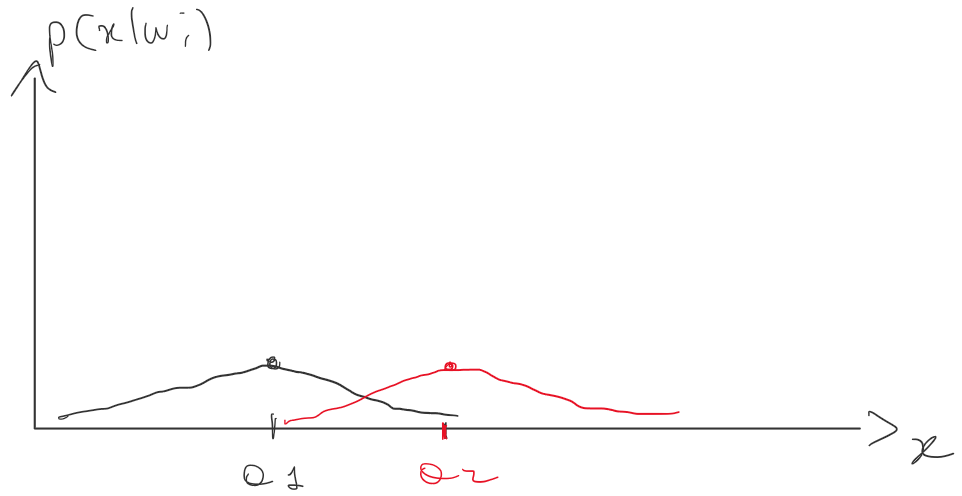
\includegraphics[scale=0.35]{C_10_1}
    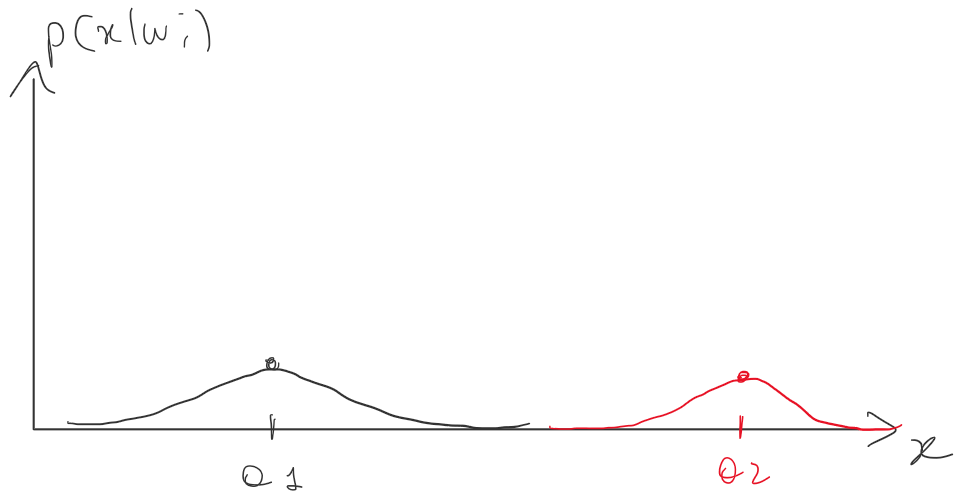
\includegraphics[scale=0.35]{C_10_2}
    \centering
\end{figure}